% =====================================================================
% A2 — Section 4: Results.  DRAFT 1, 6 Oct 2026.
% One subsection per claim, verdict in the first sentence. Numbers
% recomputed from results/fig4a and results/fig4b on 6 Oct.
% =====================================================================
\section{Results}
\label{sec:results}



\subsection{C1: the training-free prediction}
\label{sec:res-c1}

C1 reproduces and Fig.~\ref{fig:c1} shows the fraction of random training sets
with $\lambda_3 > 0$. It is zero up to $r \approx 0.27$, then rises steep and
passes 0.5 at $r = 0.41$, very close to the $r_c \approx 0.4$ reported in the
paper. My own implementation and the authors' code agree on all 1800 training sets that I checked with both. Among training sets with $\lambda_3 > 0$, the
median $\lambda_3$ also grows steadily with $r$, so according to the theory
more data should mean faster learning.

\subsection{C2: steps to $\mathrm{RQI} > 0.95$}
\label{sec:res-c2}

C2 does not reproduce with the released configuration. I first checked that I am running the same experiment as the authors. For their three seeds, the steps to $\mathrm{RQI} > 0.95$ in my runs match the values saved in their repository in all 33 runs, so the setup reproduces their runs exactly.

With twenty seeds per size the picture changes (Fig.~\ref{fig:c2}a,b). No run
finds the structure below $r = 0.45$. When moving above that success becomes more likely
only slowly, and 10\% of runs succeed at $r = 0.45$, 40\% at $r = 0.73$, and all
of them only at $r = 0.98$. The fraction of successful runs passes half only at $r \approx 0.76$,
while the theory's curve does so at $r = 0.41$ (Fig.~\ref{fig:c2}b).

None of the 82 runs with $\lambda_3 = 0$ found the structure, which is consistent with the
theory. But only 70 of the 138 runs with $\lambda_3 > 0$ did. In my runs, having
enough parallelograms in the training set was necessary, but not sufficient.

The failed runs do not seem to be just slow. I retrained ten of them, all with
$\lambda_3 > 0$, for $5 \times 10^4$ steps. None reached the threshold, and in nine of
them RQI did not change at the saved checkpoints after step 5000 (final
values 0.06-0.57).

My runs also look different from the published Fig.~4(b). Here, failures
stop around $r \approx 0.55$, and successful runs need about 150-550 steps,
fewer with more data. Most of mine need between about 650 and 1200 steps,
whatever the value of $r$. The authors' own saved results for the released script look like mine, not like the published panel. 
Since the paper does not say which settings were used for
that panel, the reason for the difference is unclear.

% Ablation figure defined here so that it lands next to Sec. 5.
\begin{figure*}[t]
  \centering
  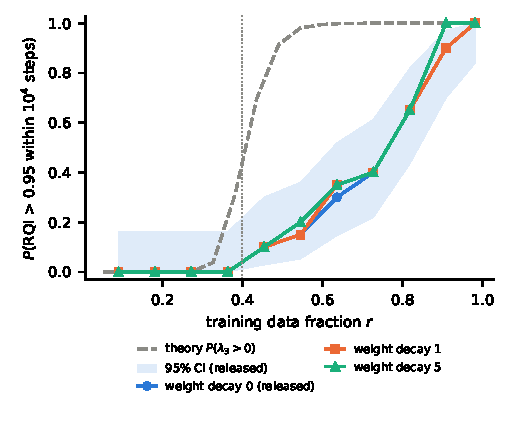
\includegraphics[width=0.49\textwidth]{figures/ablation_wd}\hfill
  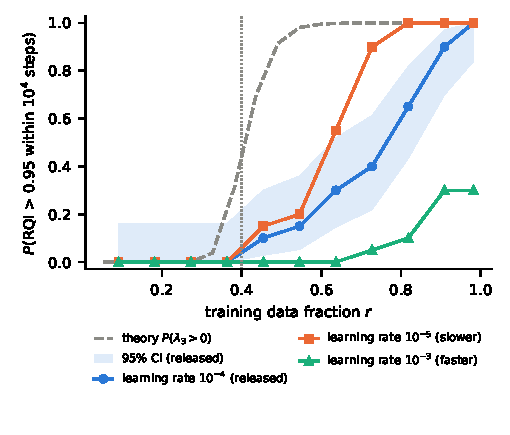
\includegraphics[width=0.49\textwidth]{figures/ablation_lrdec}
  \caption{Fraction of runs reaching $\mathrm{RQI}>0.95$ within $10^4$ steps
  under the two ablations, 220 runs per setting on the same training sets.
  The dashed line shows the theory's $\Pr(\lambda_3>0)$. To the left is the decoder weight decay (A1).
  And to the right is the decoder learning rate (A2).}
  \label{fig:ablations}
\end{figure*}

\subsection{C3: dependence on the grokking rate}
\label{sec:res-c3}

C3 does not reproduce either. The claim is that the time towards the linear structure scales like $1/\lambda_3$, so runs with a larger $\lambda_3$ should succeed sooner. Among the
70 successful runs there is no such trend (Fig.~\ref{fig:c2}c). The Spearman
correlation between steps and $\lambda_3$ is 0.15, and the
log-log slope is $-0.03$ instead of $-1$. The paper's Fig.~5(b) also shows runs with
$\lambda_3 > 0$ that fail within $10^4$ steps, which its text does not discuss.
